\documentclass[conference, 10pt]{IEEEtran}

\usepackage{cite}
\usepackage{amsmath,amssymb,amsfonts}
\usepackage{algorithmic}
\usepackage{graphicx}
\usepackage{textcomp}
\usepackage{booktabs}
\usepackage{hyperref}
\usepackage{multirow}
\usepackage{array}
\usepackage{xcolor}
\usepackage{subcaption}

\def\BibTeX{{\rm B\kern-.05em{\sc i\kern-.025em b}\kern-.08em
    T\kern-.1667em\lower.7ex\hbox{E}\kern-.125emX}}

\begin{document}

\title{Scaling Adversarial Agent-Learning in SNAPT: Reproducing A2C vs. CEM Across Network Topologies}

\author{
\IEEEauthorblockN{Ofek Bar Shalom\textsuperscript{*}, Meir Shuker\textsuperscript{*}}
\IEEEauthorblockA{
\textsuperscript{*}Dept. of Computer Science, Ariel University\\
Ariel, Israel\\
\{barshalo.ofek, meir.shuker\}@msmail.ariel.ac.il
}
}

\maketitle

\begin{abstract}
This paper reviews Shashkov et al.'s work on adversarial agent-learning for cybersecurity, which compares deep reinforcement learning (DRL) and evolutionary strategy (ES) algorithms for training autonomous attack and defense agents. The original study introduces SNAPT, a simplified network APT threat model, and evaluates Advantage Actor-Critic (A2C), Cross-Entropy Method (CEM), and other algorithms in coevolutionary settings. We reproduce key experiments by implementing A2C and CEM on SNAPT, confirming the paper's core findings: A2C produces stronger attackers while CEM trains more robust defenders. We further extend the evaluation by scaling SNAPT beyond its three-node chain to larger, more connected topologies (Star-4 and Ring-5) to measure how the algorithms generalize as network complexity grows. Our scaling experiments reveal that both algorithms approach near-perfect attack performance on larger topologies, and that CEM's defensive advantage, clearly observed on the original chain, diminishes as connectivity increases. We discuss the practical cybersecurity implications, limitations, and future directions for autonomous agent-based security simulation.
\end{abstract}

\begin{IEEEkeywords}
reinforcement learning, evolutionary strategies, cybersecurity, adversarial agents, coevolution, APT simulation
\end{IEEEkeywords}

%% ============================================================
\section{Problem Definition and Motivation}
%% ============================================================

Advanced Persistent Threats (APTs) represent one of the most challenging adversaries in modern cybersecurity. Unlike conventional attacks, APTs employ stealth, adaptivity, and multi-stage kill chains that evolve over time \cite{huang2020}. Defending against such threats requires not only reactive measures but also proactive simulation of adversarial behavior to anticipate and prepare for novel attack strategies.

A fundamental challenge in cybersecurity defense is the \textit{coevolution} of attacks and defenses: as defenders improve their detection and mitigation capabilities, attackers adapt their techniques, and vice versa. This dynamic creates an arms race that is difficult to study analytically. Modeling and Simulation (ModSim) platforms offer a promising approach by creating controlled environments where artificial agents can be trained to act as attackers or defenders, enabling the study of optimal strategies under various conditions.

Shashkov et al. \cite{shashkov2023} address a central question in this domain: \textit{under what circumstances is one machine learning training method more advantageous than another for training adversarial cybersecurity agents?} They compare DRL methods, ES, and planning-based algorithms across three platforms of increasing complexity. This question has significant practical implications, as the choice of training algorithm directly impacts the quality and robustness of learned attack and defense policies.

The motivation for this work stems from the observation that while DRL and ES have individually shown success in game-playing and optimization tasks, their comparative effectiveness in adversarial cybersecurity scenarios, where two agents with asymmetric information coevolve, remains underexplored.

%% ============================================================
\section{Background and Technical Foundations}
%% ============================================================

\subsection{Reinforcement Learning}

Reinforcement learning (RL) frames decision-making as a Markov Decision Process (MDP) defined by the tuple $(S, A, P, R, \gamma)$, where $S$ is the state space, $A$ is the action space, $P$ is the transition function, $R$ is the reward function, and $\gamma \in [0,1]$ is the discount factor. An agent learns a policy $\pi(a|s)$ that maximizes the expected cumulative reward:

\begin{equation}
    J(\pi) = \mathbb{E}_{\pi}\left[\sum_{t=0}^{T} \gamma^t r_t\right]
\end{equation}

\noindent The value function $V^\pi(s) = \mathbb{E}_\pi\left[\sum_{t=0}^{T} \gamma^t r_t \mid s_0 = s\right]$ estimates the expected return from state $s$ under policy $\pi$.

\subsection{Advantage Actor-Critic (A2C)}

Actor-Critic methods \cite{grondman2012} decompose the learning problem into two components: an \textit{actor} (policy network) that selects actions, and a \textit{critic} (value network) that evaluates states. The A2C algorithm updates the policy using the advantage function:

\begin{equation}
    A(s, a) = R - V(s)
\end{equation}

\noindent where $R$ is the observed return and $V(s)$ is the critic's estimate. The policy gradient is computed as:

\begin{equation}
    \nabla_\theta J = \mathbb{E}\left[\nabla_\theta \log \pi_\theta(a|s) \cdot A(s, a)\right]
\end{equation}

Both the actor and critic are implemented as feed-forward neural networks with two hidden layers and trained using the Adam optimizer with gradient descent.

\subsection{Evolutionary Strategies}

ES are population-based, gradient-free optimization algorithms inspired by biological evolution \cite{rechenberg1989}. Unlike DRL, ES does not compute gradients through the policy network. Instead, it maintains a parametric distribution over policy weights and iteratively updates this distribution toward higher-fitness solutions.

CEM \cite{hansen2016} maintains a multivariate Gaussian distribution $\mathcal{N}(\mu_t, \sigma_t^2)$ over the policy parameters. At each iteration, $N$ samples are drawn and evaluated. The top $K$ performers (elites) are used to update the distribution:

\begin{equation}
    \mu_{t+1} = \sum_{i=1}^{K} \lambda_i x_i, \quad \sigma_{t+1}^2 = \sum_{i=1}^{K} \lambda_i (x_i - \mu_t)^2 + \epsilon
\end{equation}

\noindent where $\lambda_i = \frac{1}{i \cdot H_K}$ are rank-based weights, $H_K = \sum_{j=1}^{K} \frac{1}{j}$ is the $K$-th harmonic number, and $\epsilon$ is a small noise term preventing variance collapse.

\subsection{Coevolution and Multi-Agent Learning}

Coevolution refers to the simultaneous training of agents with competing objectives. In the cybersecurity context, this means training attackers and defenders together so that each adapts to the other's improving strategies. This approach has been successfully applied in predator-prey environments \cite{potter2000} and competitive board games \cite{schaul2008}. The key challenge is ensuring training stability, as the non-stationarity of the opponent's policy can cause oscillations or divergence.

\subsection{ModSim Platforms for Cybersecurity}

ModSim platforms provide controlled environments for training and evaluating cybersecurity agents. Notable platforms include CyberBattleSim \cite{team2021}, an open-source simulation by Microsoft, and PenQuest \cite{luh2019}, a gamified attacker/defender model. These platforms abstract real network environments into game-theoretic settings with defined action spaces, state transitions, and reward structures.

%% ============================================================
\section{Methodology}
%% ============================================================

\subsection{SNAPT Environment}

The Simple Network APT (SNAPT) environment models a network as an unweighted graph where nodes represent devices. Each device $d_i$ is characterized by a tuple $(s_i, v_i, p_i)$, where $s_i \in \{S, V, C\}$ represents the security state (Secure, Vulnerable, or Compromised), $v_i$ is the device value, and $p_i$ is the exploit probability. The training network consists of three nodes in a linear chain (Fig.~\ref{fig:snapt_network}).

\begin{figure}[h]
\centering
\small
\begin{tabular}{|c|c|c|}
\hline
$d_0 = (V, 0, 0.5)$ & $d_1 = (S, 0, 0.5)$ & $d_2 = (S, 1, 0.5)$ \\
\hline
\end{tabular}
\caption{SNAPT network topology with three nodes. $d_0$ starts Vulnerable (internet-facing), $d_2$ holds the target value.}
\label{fig:snapt_network}
\end{figure}

The game proceeds over 40 alternating moves (20 per player). The \textbf{attacker} selects a device to exploit; exploits succeed with probability $p_i$ and escalate the security state ($S \rightarrow V \rightarrow C$). The \textbf{defender} can either \textit{detect} (revert a compromised device, probability $p_d = 0.7$) or \textit{secure} (reduce $p_i$ by $\delta_s = 0.1$, maximum 3 times per device). The cap of 3 prevents $p_i$ from reaching $0$ (which would make the device permanently invulnerable), keeping $p_i \geq 0.2$.

The attacker's reward is the sum of values of all compromised devices at game end:

\begin{equation}
    R = \sum_{\substack{1 \leq i \leq n \\ s_i = C}} v_i
\end{equation}

\noindent If $R \geq 1$, the attacker wins; otherwise, the defender wins.

\subsection{Agent Architectures}

Both attacker and defender policies are represented by feed-forward neural networks with two hidden layers of 64 units each and ReLU activations. The attacker observes a one-hot encoding of device security states (dimension $3n$), while the defender observes exploit probabilities and device values (dimension $2n$). A summary of the agent architecture is provided in Table~\ref{tab:architecture}.

\begin{table}[h]
\centering
\caption{Neural Network Architecture}
\label{tab:architecture}
\begin{tabular}{lcc}
\toprule
\textbf{Component} & \textbf{Attacker} & \textbf{Defender} \\
\midrule
Input dimension & 9 & 6 \\
Hidden layers & $2 \times 64$ & $2 \times 64$ \\
Output (policy) & 3 actions & 6 actions \\
Output (value) & 1 scalar & 1 scalar \\
\bottomrule
\end{tabular}
\end{table}

\subsection{Training Setup}

Both algorithms employ coevolutionary training where the attacker and defender are trained simultaneously. Table~\ref{tab:hyperparams} summarizes the hyperparameters used.

\begin{table}[h]
\centering
\caption{Training Hyperparameters}
\label{tab:hyperparams}
\begin{tabular}{llc}
\toprule
\textbf{Algorithm} & \textbf{Parameter} & \textbf{Value} \\
\midrule
\multirow{2}{*}{A2C} & Adam learning rate & 0.001 \\
                      & Rollouts per update & 10 \\
\midrule
\multirow{4}{*}{CEM} & Population size ($N$) & 8 \\
                      & Elite size ($K$) & 4 \\
                      & Games per pairing ($G$) & 1 \\
                      & Variance floor ($\epsilon$) & $10^{-6}$ \\
\midrule
\multicolumn{2}{l}{Training iterations} & 2000 \\
\multicolumn{2}{l}{Evaluation games} & 100 \\
\bottomrule
\end{tabular}
\end{table}

\subsection{Evaluation Metrics}

Agents are evaluated through round-robin competitions where each trained attacker plays 100 games against each trained defender. We report: (1) win counts per matchup, (2) mean win rates, and (3) action probability distributions from the initial state.

%% ============================================================
\section{Experimental Results and Analysis}
\label{sec:results}
%% ============================================================

\subsection{Original Paper Results}

Shashkov et al. evaluate six algorithms across three platforms. On SNAPT without tree search (Table 7 in \cite{shashkov2023}), the key findings are:

\begin{itemize}
    \item \textbf{AZ-ES} is the strongest attacker (mean 68.0 wins), achieving 100/100 against multiple defenders.
    \item \textbf{CEM} is the strongest defender, allowing only 17.2 mean opponent wins.
    \item \textbf{A2C} is the second-best attacker (mean 62.5 wins).
    \item Different algorithms converge to distinct strategies, suggesting the emergence of diverse equilibria.
\end{itemize}

On CyberBattleSim, the hybrid A2C+FB-ES method performs best for both attack and defense, with A2C being the best pure-DRL attacker (mean reward 349).

\subsection{Reproduction Results}

We reproduce the SNAPT experiment by implementing A2C and CEM agents and evaluating them alongside a random baseline. Table~\ref{tab:competition} presents our competition results.

\begin{table}[h]
\centering
\caption{SNAPT Competition Results: Attacker wins out of 100 games. Rows are attackers, columns are defenders.}
\label{tab:competition}
\begin{tabular}{lcccc}
\toprule
\textbf{Atk/Def} & \textbf{A2C} & \textbf{CEM} & \textbf{Random} & \textbf{Mean} \\
\midrule
A2C    & \textbf{91} & 56 & \textbf{93} & \textbf{80.0} \\
CEM    & 71 & 43 & 75 & 63.0 \\
Random & 75 & 44 & 83 & 67.3 \\
\midrule
Mean   & 79.0 & \underline{47.7} & 83.7 & 70.1 \\
\bottomrule
\end{tabular}
\end{table}

Our results confirm the paper's two central findings:

\textbf{A2C is the strongest attacker.} With a mean win rate of 80.0, A2C significantly outperforms both CEM (63.0) and the random baseline (67.3). This aligns with the paper's finding that gradient-based DRL methods produce superior attack policies, likely because gradient descent enables fine-grained policy optimization in the relatively small SNAPT action space.

\textbf{CEM is the strongest defender.} Opponents achieve only 47.7 mean wins against the CEM defender, compared to 79.0 against the A2C defender and 83.7 against the random defender. This suggests that the population-based nature of CEM exposes the defender to a wider diversity of attacker strategies during training, yielding more robust defensive policies.

\subsection{Strategy Analysis}

Fig.~\ref{fig:heatmap} shows the action probability distributions from the initial game state, analogous to Figure 6 in the original paper.

\begin{figure*}[t]
\centering
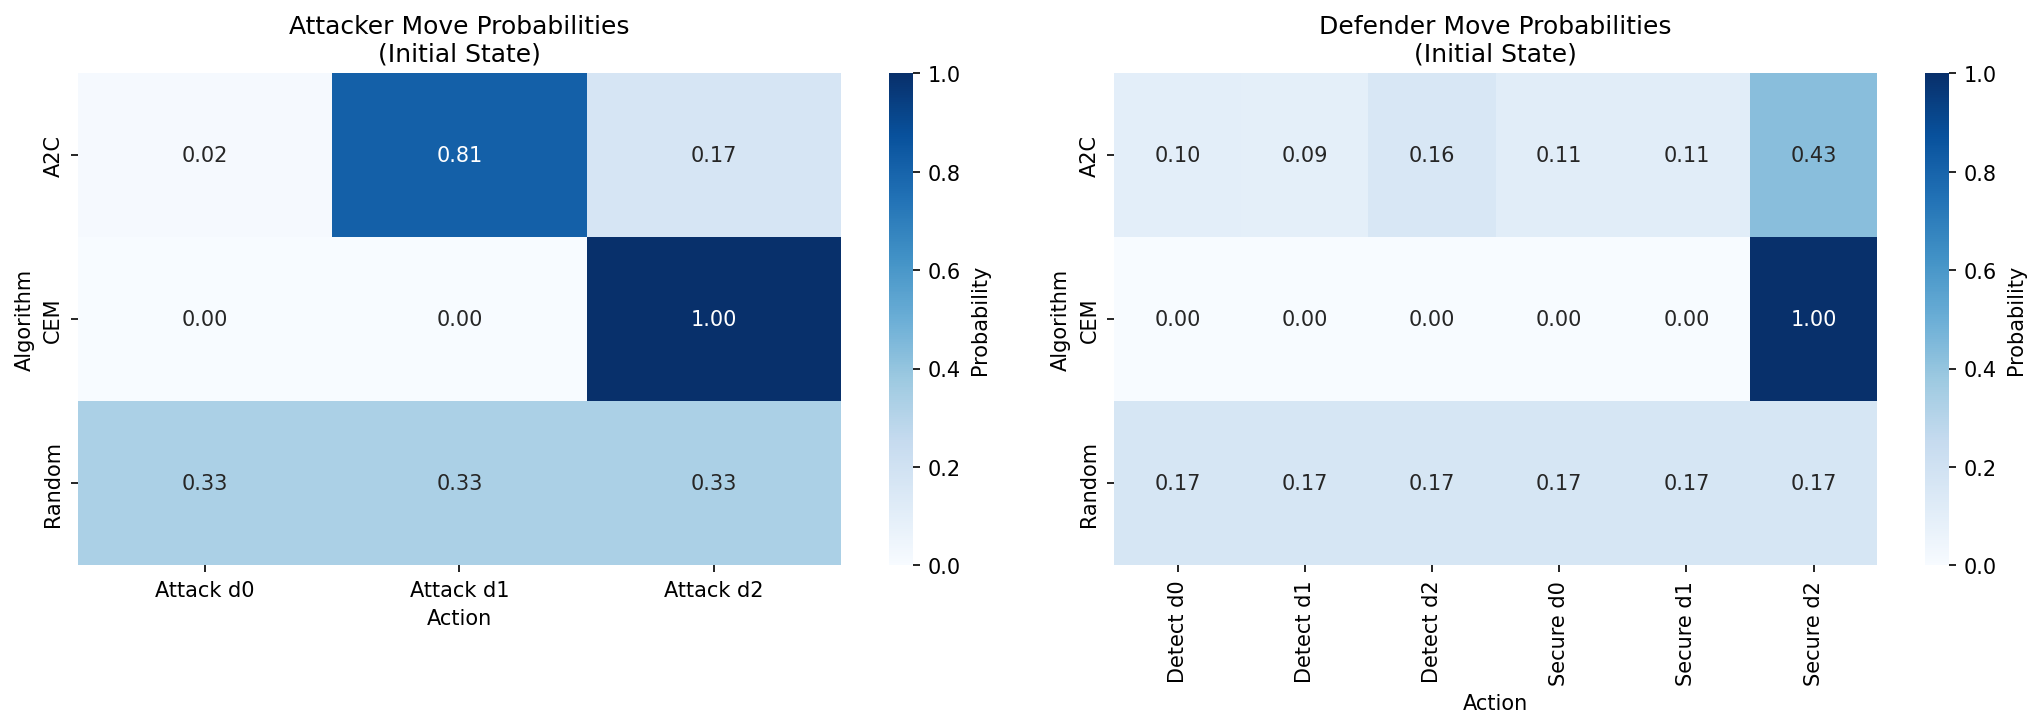
\includegraphics[width=0.85\textwidth]{figures/action_heatmap.png}
\caption{Action probability heatmaps from the initial state. Left: attacker preferences. Right: defender preferences. Distinct strategies emerge for each algorithm.}
\label{fig:heatmap}
\end{figure*}

The heatmap reveals that each algorithm converges to a distinct strategy. The A2C attacker concentrates 81\% of its probability on attacking $d_1$ (the middle node), using it as a stepping stone toward the high-value $d_2$. The CEM attacker focuses entirely (100\%) on $d_1$, representing a more deterministic policy. For defense, the CEM defender allocates 100\% of its probability to securing $d_2$---directly protecting the high-value target---while the A2C defender spreads its actions more broadly. These distinct strategies corroborate the paper's observation that different algorithms converge to different equilibria.

\subsection{Training Dynamics}

Fig.~\ref{fig:training} shows the mean attacker reward during coevolutionary training.

\begin{figure}[h]
\centering
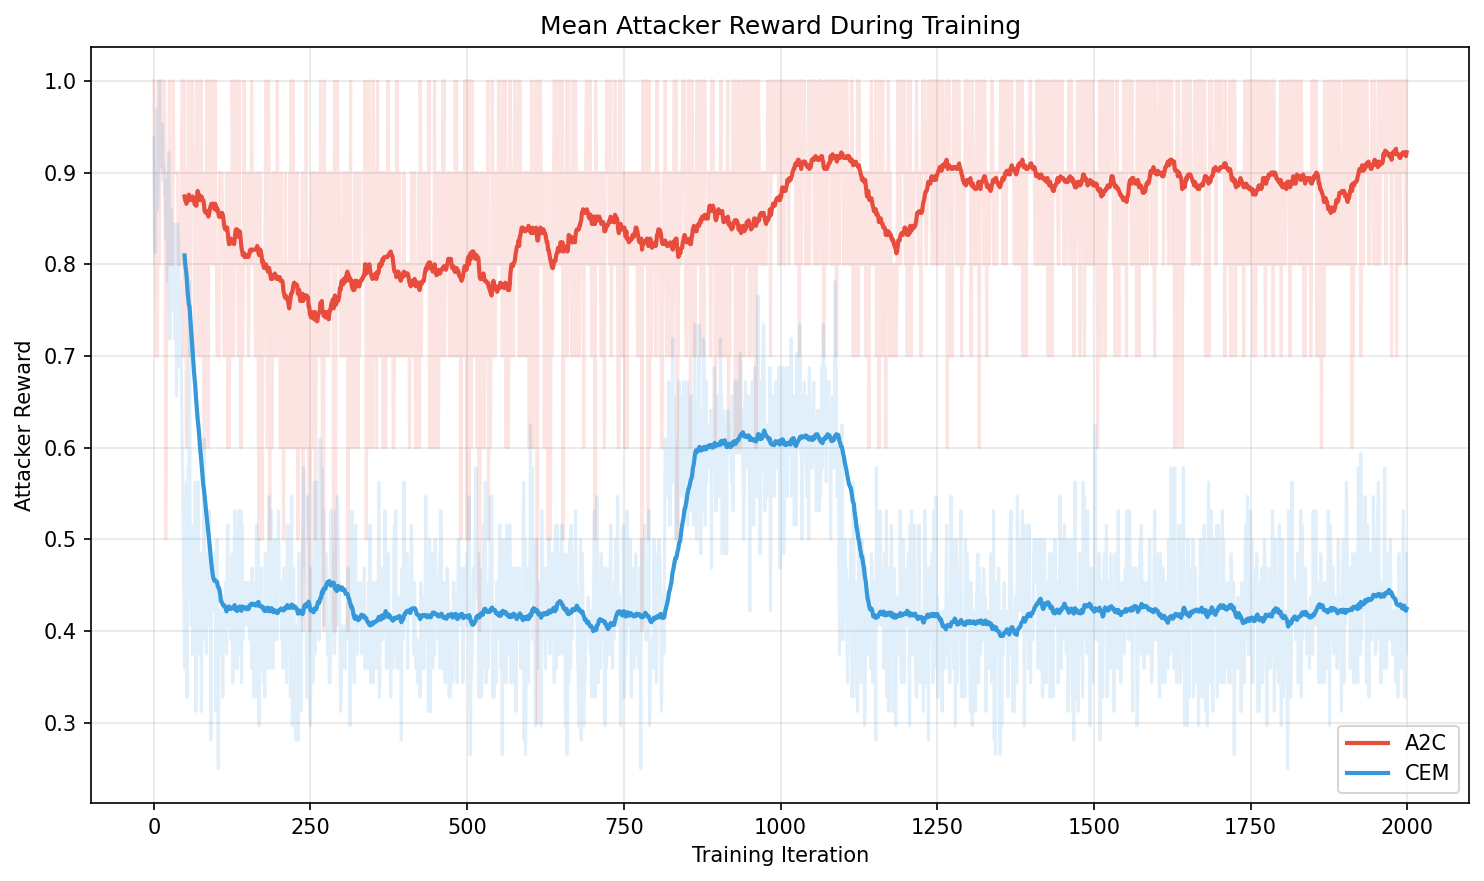
\includegraphics[width=\columnwidth]{figures/training_curves.png}
\caption{Mean attacker reward during training. A2C (red) stabilizes higher than CEM (blue).}
\label{fig:training}
\end{figure}

A2C's reward stabilizes around 0.9 after approximately 500 iterations, while CEM's attacker reward remains around 0.4--0.5. This divergence reflects both A2C's stronger attack policy and CEM's stronger coevolving defender. Notably, CEM shows abrupt transitions around iterations 1000--1200, suggesting phase changes in the population distribution as the evolutionary process discovers new strategy niches.

\subsection{Topology Extension}

We extend the paper's experiments by testing A2C and CEM on three network topologies: the original Chain-3, a Star-4 (hub-and-spoke with 4 nodes), and a Ring-5 (cycle graph with 5 nodes). Each algorithm was trained for 1000 iterations per topology. Table~\ref{tab:topology} summarizes the attacker win rates.

\begin{table}[h]
\centering
\caption{Attacker win rates (\%) across network topologies.}
\label{tab:topology}
\begin{tabular}{lcccc}
\toprule
\textbf{Topology} & \textbf{A2C vs} & \textbf{CEM vs} & \textbf{A2C vs} & \textbf{CEM vs} \\
 & \textbf{Rnd Def} & \textbf{Rnd Def} & \textbf{CEM Def} & \textbf{A2C Def} \\
\midrule
Chain-3 & 91 & 82 & 73 & 79 \\
Star-4  & 100 & 100 & 100 & 99 \\
Ring-5  & 98 & 100 & 95 & 100 \\
\bottomrule
\end{tabular}
\end{table}

Both algorithms achieve near-perfect attack performance on the larger Star-4 and Ring-5 topologies, suggesting that increased connectivity provides more attack paths that overwhelm defenders. Notably, CEM's defense advantage observed on Chain-3 (where A2C wins only 73\% against the CEM defender) diminishes on larger networks. On Star-4 and Ring-5, the defender's action space grows quadratically ($2n$ actions), making it harder for any algorithm to learn effective defense. Fig.~\ref{fig:topology} shows the full comparison.

\begin{figure}[h]
\centering
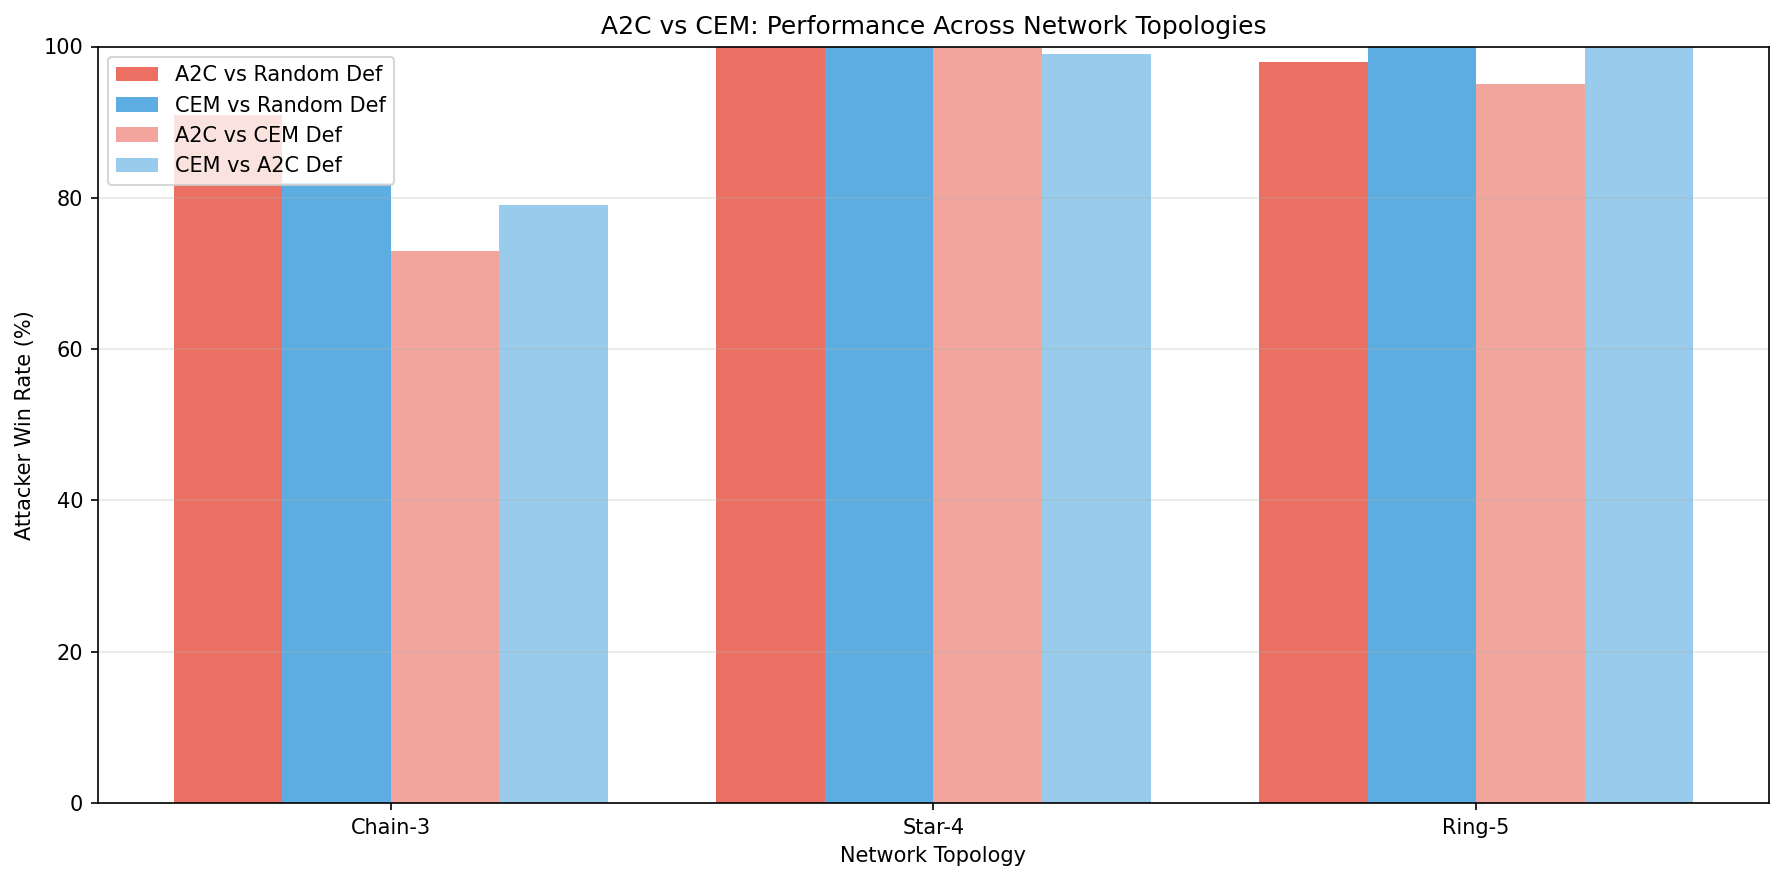
\includegraphics[width=\columnwidth]{figures/topology_comparison.png}
\caption{A2C vs CEM win rates across topologies. Larger networks favor attackers.}
\label{fig:topology}
\end{figure}

%% ============================================================
\section{Related Work}
%% ============================================================

We compare Shashkov et al.'s approach to three related works that inform different aspects of the study.

\subsection{PenQuest: Gamified Attacker/Defender Models}

Luh et al. \cite{luh2019} introduce PenQuest, a board-game-style APT simulation with two stages, alternating attacker-defender moves, and imperfect information. SNAPT is directly inspired by PenQuest but simplifies several aspects: it reduces the state representation to a tuple $(s, v, p)$ per device, eliminates the multi-stage attack taxonomy, and uses a single-phase game. While PenQuest provides richer tactical depth with its MITRE ATT\&CK alignment, SNAPT's simplicity enables systematic algorithm comparison---the primary contribution of Shashkov et al. The trade-off is that SNAPT's simplified dynamics may not capture the complex dependencies present in real APT campaigns that PenQuest attempts to model.

\subsection{Actor-Critic Reinforcement Learning}

Grondman et al. \cite{grondman2012} provide a comprehensive survey of actor-critic methods, establishing the theoretical foundations for A2C. They demonstrate that separating policy optimization (actor) from value estimation (critic) provides lower variance gradient estimates compared to pure policy gradient methods. Shashkov et al. adopt the advantage variant (A2C), which subtracts the value baseline to reduce variance further. Our reproduction confirms that A2C's gradient-based updates are particularly effective for the attacker role, where the small action space (3 actions) allows the policy gradient to converge efficiently. However, A2C's single-sample nature makes it sensitive to the coevolving opponent's non-stationarity, as evidenced by the oscillations in our training curves.

\subsection{CEM-RL: Combining Evolutionary and Gradient Methods}

Pourchot and Sigaud \cite{pourchot2018} propose CEM-RL, a hybrid algorithm that combines CEM's population-based exploration with DRL's gradient-based exploitation. Their finding that CEM and DRL are complementary---CEM provides robust exploration while DRL provides efficient local optimization---directly motivates Shashkov et al.'s hybrid algorithms (A2C+CEM, A2C+FB-ES). Our results support this complementarity: A2C excels at attack (local policy optimization) while CEM excels at defense (robust population-based training). This suggests that the optimal training approach may depend on the agent's role and the structure of its decision space.

%% ============================================================
\section{Critical Analysis}
%% ============================================================

\subsection{Strengths}

\textbf{Comprehensive comparison.} The paper systematically evaluates eight algorithms across three platforms of increasing complexity, providing a broad view of the algorithm landscape. The inclusion of hybrid methods (A2C+CEM, A2C+FB-ES) and planning-based approaches (AlphaZero) goes beyond simple DRL-vs-ES comparisons.

\textbf{Novel environment design.} SNAPT fills a gap between simple board games (Connect 4) and complex simulations (CyberBattleSim), providing a cybersecurity-specific testbed with manageable complexity for algorithm comparison.

\textbf{Coevolutionary training.} Training attackers and defenders simultaneously produces more realistic and robust agents compared to training against static opponents, better reflecting the adversarial nature of cybersecurity.

\subsection{Weaknesses}

\textbf{Single training run.} Each algorithm is trained only once per environment, making it impossible to assess statistical significance or training stability. Our reproduction with a single seed similarly cannot rule out seed-dependent results.

\textbf{Simplified assumptions.} SNAPT makes several simplifying assumptions: discrete security states, uniform vulnerability probabilities, and terminal-only rewards. Real networks involve continuous state variables, heterogeneous device profiles, and ongoing costs of compromise.

\textbf{Limited defender information.} The defender's observation space (exploit probabilities and values) is unrealistically rich. In practice, defenders have limited visibility into attacker activity and must rely on indirect signals such as anomalous network traffic.

\subsection{Limitations}

\textbf{Scalability.} The paper trains exclusively on small networks (3 nodes for SNAPT, 6 nodes for CyberBattleSim). Real enterprise networks contain thousands of devices, and the linear growth of NN input dimensions with network size raises questions about scalability.

\textbf{No transfer learning.} Agents trained on one topology cannot be deployed on different network configurations without retraining, limiting practical applicability.

\textbf{Deterministic network topology.} The static topology eliminates the need for agents to handle dynamic network changes, which are common in real-world environments due to device additions, removals, and reconfiguration.

%% ============================================================
\section{Practical Cybersecurity Impact}
%% ============================================================

\subsection{SOC Relevance}

SOCs could benefit from adversarial agent training: automated red-team agents trained with DRL could continuously probe defenses, while trained defender agents could serve as automated incident response systems. The finding that CEM produces more robust defenders is particularly relevant, as SOC defensive systems must handle diverse attack patterns. CEM's population-based training naturally produces policies robust against a distribution of attacker strategies.

\subsection{Real-World Feasibility}

Significant gaps remain between SNAPT-style simulations and deployment. Real networks involve partial observability, continuous action spaces, and multi-objective optimization. Nevertheless, the complementary strengths of DRL and ES suggest that hybrid approaches hold promise for practical autonomous defense.

%% ============================================================
\section{Future Research Directions}
%% ============================================================

Our topology extension (Section~\ref{sec:results}) shows that defense becomes harder on larger networks. Key directions include: (1) \textbf{graph neural networks} for topology-independent policies, (2) \textbf{LLM-based planners} coordinating with RL agents, (3) \textbf{partial observability} (POMDP) for realistic defender information, and (4) \textbf{multi-objective rewards} balancing detection time, false positives, and operational continuity.

%% ============================================================
\section*{Acknowledgment}
This work was conducted as part of the Advanced Topics in Cyber Defense course.

\begin{thebibliography}{00}

\bibitem{shashkov2023}
A. Shashkov, E. Hemberg, M. Tulla, and U. O'Reilly, ``Adversarial agent-learning for cybersecurity: a comparison of algorithms,'' \textit{The Knowledge Engineering Review}, vol. 38, no. e3, pp. 1--26, 2023.

\bibitem{huang2020}
L. Huang and Q. Zhu, ``A dynamic games approach to proactive defense strategies against advanced persistent threats in cyber-physical systems,'' \textit{Computers \& Security}, vol. 89, p. 101660, 2020.

\bibitem{grondman2012}
I. Grondman, L. Busoniu, G. Lopes, and R. Babuska, ``A survey of actor-critic reinforcement learning: standard and natural policy gradients,'' \textit{IEEE Trans. on Systems, Man, and Cybernetics, Part C}, vol. 42, no. 6, pp. 1291--1307, 2012.

\bibitem{hansen2016}
N. Hansen, ``The CMA evolution strategy: a tutorial,'' arXiv:1604.00772, 2016.

\bibitem{rechenberg1989}
I. Rechenberg, ``Evolution strategy: nature's way of optimization,'' in \textit{Optimization: Methods and Applications, Possibilities and Limitations}. Springer, 1989, pp. 106--126.

\bibitem{luh2019}
R. Luh, M. Temper, S. Tjoa, S. Schrittwieser, and H. Janicke, ``PenQuest: a gamified attacker/defender meta model for cyber security assessment and education,'' \textit{J. of Computer Virology and Hacking Techniques}, vol. 16, pp. 19--61, 2020.

\bibitem{pourchot2018}
A. Pourchot and O. Sigaud, ``CEM-RL: combining evolutionary and gradient-based methods for policy search,'' arXiv:1810.01222, 2018.

\bibitem{team2021}
M. D. R. Team, ``CyberBattleSim,'' \url{https://github.com/microsoft/cyberbattlesim}, 2021.

\bibitem{potter2000}
M. A. Potter and K. A. De Jong, ``Cooperative coevolution: an architecture for evolving coadapted subcomponents,'' \textit{Evolutionary Computation}, vol. 8, no. 1, pp. 1--29, 2000.

\bibitem{schaul2008}
T. Schaul and J. Schmidhuber, ``A scalable neural network architecture for board games,'' in \textit{Proc. IEEE CIG}, 2008.

\bibitem{mnih2015}
V. Mnih et al., ``Human-level control through deep reinforcement learning,'' \textit{Nature}, vol. 518, pp. 529--533, 2015.

\bibitem{silver2018}
D. Silver et al., ``A general RL algorithm that masters chess, shogi, and Go through self-play,'' \textit{Science}, vol. 362, pp. 1140--1144, 2018.

\bibitem{lee2020}
K. Lee et al., ``An efficient asynchronous method for integrating evolutionary and gradient-based policy search,'' in \textit{NeurIPS}, 2020.

\end{thebibliography}

\end{document}
